\chapter{塑闪阵列探测器分系统简介}
塑闪阵列探测器(以下将简称PSD)是暗物质粒子探测卫星的关键子探测器之一。
它的功能有两个:一是协助 BGO量能器,区分电子和光子事件;二是鉴别入射重离子(Z=1~20)的种类。

\section{工作原理}
PSD选择了\SI{10}{\milli\meter}厚的有机塑料闪烁体EJ-200~\parencite{ej-200}作为分系统的探测介质材料,通过测量入射粒子在其中的量沉积能量来实现以上两个功能需求。
有机塑料闪烁体由于具有强的抗辐照特性、快的时间响应性、好的均匀性、长的光衰减长度、光输出高且易于加工等属性,在空间探测系统中常被用于提供系统的触发信号、能量测量及飞行时间测量。
\subsection{重离子鉴别的原理}

粒子在物质中的能量损失与其能量有紧密的关系。
对于重带电粒子(质量大于电子),其平均能量损失率与入射粒子能量的关系如图~\ref{fig:ch2:energyloss_vs_velocity}所示。
在不同能量范围内,导致能量损失的主要相互作用并不一样,图~\ref{fig:ch2:energyloss_vs_velocity}中用竖直的带子区分不同的能损区域。
DAMPE关注的能量范围属于相对论能区,此时主要是电离能损和辐射能损占主导地位。
在中等能量范围内电离相互作用起主导作用,辐射效应可以忽略;随着能量的不断升高,辐射效应逐渐不断增强,并最终其占据主导地位。
而对于重离子来说,由于其质量较大,在DAMPE的能量范围内其辐射效应不明显,因此这里只考虑它们的电离能损。

当$0.1\lessapprox\beta\gamma\lessapprox1000$($\beta=v/c,\gamma=1/\sqrt{1-{\beta}^2}$)时,重带电粒子的电离能损可以用Bethe-Bloch方程准确描述(即图~\ref{fig:ch2:energyloss_vs_velocity}中的Bethe区)):
\begin{equation}\label{eq:beth_bloch}
-\left\langle\frac{dE}{dx}\right\rangle = Kz^2\frac{Z}{A}\frac{1}{{\beta}^2}
\left[\frac{1}{2}\ln\frac{2m_ec^2{\beta}^2{\gamma}^2T_{max}}{I^2}-{\beta}^2-\frac{\delta(\beta\gamma)}{2}\right]
\end{equation}
其中$-\left\langle\frac{dE}{dx}\right\rangle$表示的是粒子通过单位约化介质层厚度的平均电离能损,K为常数,Z、A是探测器介质的原子序数和质量数,z是入射粒子的电荷数,$m_e$是电子的静止质量,c是光速,I是为介质的电离常数(也称平均激发能,有效电离电位等),$T_{max}$为入射粒子与静止的电子碰撞时传递给电子的最大动能。
$\delta$是密度效应修正项。

由公式~\ref{eq:beth_bloch}可知,对同一种探测介质来说,$dE/dx$只与入射粒子的电荷量和速度有关。
如图~\ref{fig:ch2:energyloss_vs_velocity}所示,在Bethe区随着入射粒子的能量由低逐渐增高时,能量损失起初像$1/{\beta}^2$一样快速减小,然后到达一个很宽范围的极小值区域。
这个极小值区域最低点约在$\beta\gamma\approx3.2$附近,且与介质无关。
通常将此最小值处的电离能损称为最小电离,把能量损失率为最小值的粒子称为最小电离粒子(Minimum Ionizing Particles,简称MIPs)。
MIPs粒子往往用来统称$z=1$的相对论性粒子(如宇宙线$\mu$子),因为它们的能量损失率与最小电离值非常接近。
经过最小电离值之后,能量损失率开始缓慢上升,这是由于公式~\ref{eq:beth_bloch}方括号内第一项随$\ln{\beta}^2{\gamma}^2$变大,这个过程被称为相对论性上升。
随着能量的进一步升高,入射粒子的横向电场增强,靶核核外电子电荷密度的屏蔽效应也逐渐显著,减小了能量损失率,这种效应被称为密度效应。
密度效应在公式~\ref{eq:beth_bloch}中用$\delta/2$来表示,它使得电离能量损失率减缓并最终达接近一个常数值,称为费米坪(见图~\ref{fig:ch2:fermi_plateau})。

\begin{figure*}
	\centering
	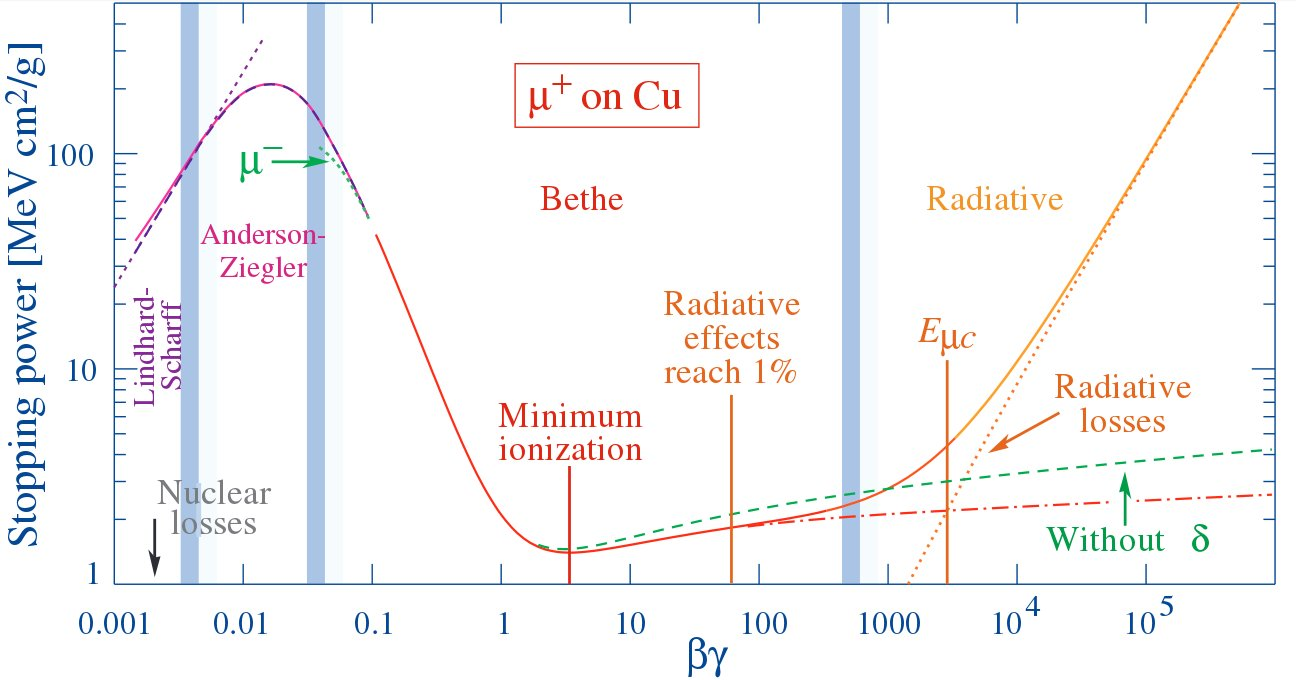
\includegraphics[width=0.8\linewidth]{chap/description/fig/energyloss_vs_velocity}
	\caption{${\mu}^+$在Cu中的能量损失率与速度的关系(用$\beta\gamma$表示),引自~\parencite{pdg_book}。 图中实线是总的能量损失率,包含了所有相互作用。}
	\label{fig:ch2:energyloss_vs_velocity}
\end{figure*}

\begin{figure*}
\centering
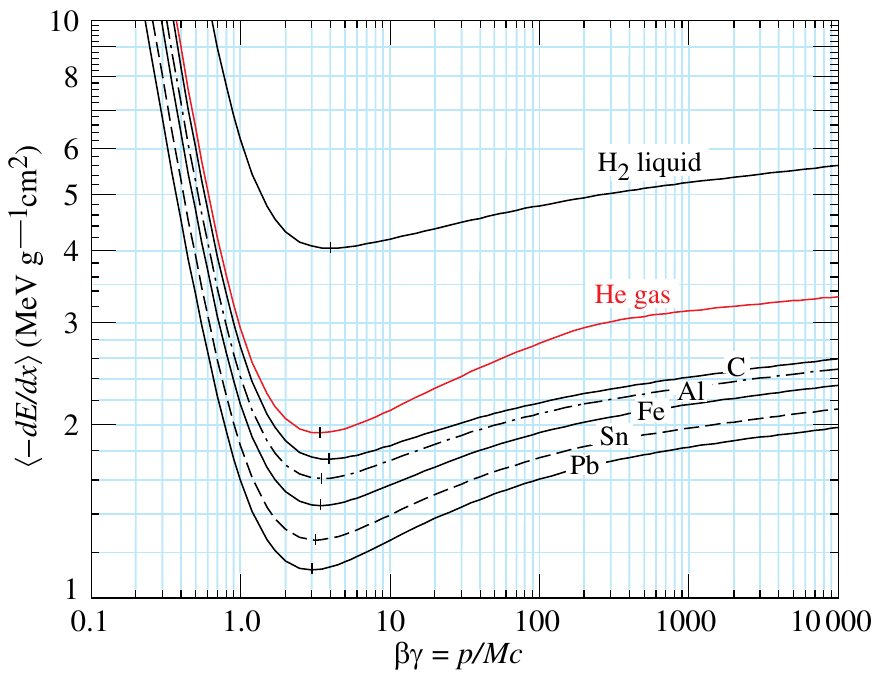
\includegraphics[width=0.8\linewidth]{chap/description/fig/fermi_plateau}
\caption{入射粒子在几种不同介质中的电离能量损失随入射粒子动量的变化,可以清楚地看到费米坪。引自~\parencite{pdg_book}。}
\label{fig:ch2:fermi_plateau}
\end{figure*}

可以看到,对于相对论粒子来说($\beta\gamma>1$),其电离能量损失虽然与速度相关,但在很大的能量范围内其变化并不大。
因此,相对论重离子的电离能损可以近似为:
\begin{equation}
-\left\langle\frac{dE}{dx}\right\rangle \propto z^2
\end{equation}
即与电荷量的平方成正比。
不同种类的核素在探测器介质中的电离能损相差巨大,因此可以通过测量沉积能量进行重离子的鉴别。
实际中,探测器的响应与沉积能量并不成正比,这会使得探测器鉴别能力变差,这个问题将在下一章中详细讨论。

\subsection{高能$e/\gamma$鉴别的原理}

光子(或$\gamma$射线)与物质的相互作用与



\section{PSD的性能要求}

\section{探测器组成}

\section{前端电子学}

\section{支撑结构}